\chapter{Analysis}

\red{CHAPTER STATUS: PLANNING/OUTLINE}

\section{Particle Identification}

\section{Data Selection}

\subsection{Spill Level Cuts}

\subsubsection{Duty Factor}

The beam structure is delivered in \emph{bunches} 
of protons separated by 18.9ns. These bunches are better
known as \emph{RF buckets}, as they are synchronized with the 18.9ns cycle of the Fermilab RF clock. Ideally, each of these RF buckets deliver a steady number of protons per bucket.

In practice however, this is not the case, and not all the RF buckets delivered are occupied within a given spill. The fraction of buckets occupied is known as the accelerator Duty Factor, \emph{DF}, and can be measured using a reference beam counter as

\begin{eqnarray} DF = \frac{\langle I \rangle ^2}{\langle I^2 \rangle} &
with &  I = \sum_{N_trig} N_{X2T}
\end{eqnarray}

where $N_X2T$ is the number of hits in the X2T 

\subsection{Dimuon Level Cuts}

\subsection{Track Level Cuta}

\subsection{Other Cuts}

\section{Dimuon Yields}


\subsection{Binning of Data}

The $x_2$ bins for this EMC ratio measurement were chosen such that each
bin in $x_2$ has similar levels of statistics. 

Concurrent with this analysis, studies of $\bar{d}(x_2)/\bar{u}(x_2)$ and 
parton energy loss are conducted. Due to the nearly
identical source of signal across these studies (good Drell-Yan target
dimuons), a consistent selection of kinematic binning maintains a 
certain continuity among analyses. The $x_2$ binning chosen can be found in Table \ref{tab:x2bins}

\begin{table}
	\centering
	\setlength\tabcolsep{4pt}
\begin{minipage}{0.48\textwidth}
	\centering
	\begin{tabular}{ll}
		\toprule
		Bin\# & $x_2$ Range\\
		\midrule
		0 & (0.08, 0.14] \\
		1 & (0.14, 0.16] \\
		2 & (0.16, 0.18] \\
		3 & (0.18, 0.21] \\
		4 & (0.21, 0.25] \\
		5 & (0.25, 0.31] \\
		6 & (0.31, 0.53] \\
		\bottomrule
	\end{tabular}
	\caption{$x_2$ bin ranges}
	\label{tab:x2bins} 
\end{minipage}%
\hfill
\begin{minipage}{0.48\textwidth}
	\centering
	\begin{tabular}{ll}
		\toprule
		target & yield \\ 
		\midrule
		None   &  104 \\
		Empty  &  84 \\
		LH2    &  3138 \\
		LD2    &  3472 \\
		C      &  1721 \\ 
		Fe     &  1370 \\
		W      &  1553 \\
		\bottomrule
	\end{tabular}
	\caption{Raw dimuon yields for Roadset 57} 
	\label{tab:targyields} 
\end{minipage}
\end{table}

\subsection{Raw Yields}

The total number of target Drell-Yan events recorded for each target can be found in Table
\ref{tab:targyields}. The number of events broken down into 

\section{Dimuon Weights and Corrections}

Weighting of events is a standard procedure for mapping one distribution onto another. The most common example is with Monte Carlo (MC) simulation weighting. A simple physics event MC meant to simulate a well-defined process will `throw' an event with certain kinematics randomly drawn from known distributions via \emph{inverse transform sampling}. By doing this, the simulation is already close to being physical, but according to the cross section of a given process, a certain combination of kinematics will be decidedly more or less probable. A weighting subroutine calculates this likelihood for each event and assigns a weight with respect to how likely that event is based on the kinematics thrown. When binning this weighted data, the adjusted number of events in a bin is given by
\begin{equation}
	N_{bin} = \sum_{i \in bin} w_i\ \ ;\ \ \sigma_{bin} = \sqrt{\sum_{i\in bin} w_i^2}
	\label{eq:gmc-weight}
\end{equation}
which reduces to the Poissonian statistical picture when all weights are 1.

Weighting in this manner can be used in any case where it is desirable to map one distribution to another, as in the case of applying corrections in the case of efficiencies and background subtractions. The most intuitive connection between the use of weights and corrections is in the case of efficiency corrections. Let us say that a dimuon with a certain set of kinematics, for whatever combination of effects, has a reconstruction efficiency of 80\%. This means that four out of five actual dimuons with these kinematics will be reconstructed. If you know this efficiency $\epsilon_{recon}$, you can apply a weight as $w = 1/\epsilon_{recon}$ to each dimuon, as each dimuon represents, in part, a larger population that is not fully represented. In the case of our example, a single dimuon represents $1/0.80 = 1.25$ dimuons in order to make up for the ones that are missed due to that specific inefficiency.

At SeaQuest, there is an issue of rate dependence, and as the sources of this effect is identified, we apply a correction for each source in the form of an applied weight. Here, we discuss the reconstruction efficiency and empty/none target background subtraction corrections.

\subsection{``kEfficiency'' Correction Using Messy/Clean Data}

It is a matter of combinatorics at SeaQuest that, as the intensity increases, the number of background hits on all of the detectors increases. As the number of hits in all the detectors increases, the harder it become for the tracking to identify the actual dimuon(s) from the whole event. This is regarded to be an intensity-dependent tracking efficiency. Seeing as the primary tracking algorithm for SeaQuest is kTracker, this is known as the ``kEfficiency'', and its intensity, target, and kinematic dependency makes it a factor to model and correct for.

The procedure developed by Evan McClellan of UIUC for calculating this kEfficiency is to take compare the performance of the tracking on a clean MC sample of dimuons to an analogous sample that's mixed in with real intensity-dependent background. To do this, a \emph{single} sample of MC-generated dimuons and all of their hits is generated; this sample is denoted as the \emph{``clean''} sample. Then, this sample is mixed with all of the hits from a NIM3 event from the experimental data. The NIM3 trigger, as is discussed in Chapter~2, is the randoms trigger, and by using these events we avoid any effects due to trigger selection bias. This mix of MC dimuons and NIM3 triggered data is denoted as the \emph{``messy''} sample. These NIM3 events all have an intensity, and by embedding a clean MC dimuon into a situation typical of an event at a given intensity, we get a basis by which to judge how efficiently the tracking can reconstruct a dimuon in the clean sample versus the messy sample as a function of intensity (and other kinematic variable).

It is important to note that the DY cross section is so small that there is a negligible chance that a given randomly-triggered NIM3 event will contain an actual dimuon, nonetheless a dimuon matching the characteristics of the MC dimuon that is embedded. As such, it is assumed that the dimuon embedded in the NIM3 event is the only dimuon to find in the event. It is also justified to assume that the kinematics of a dimuon is in no way correlated to the intensity, and the intensity of an event relates only to the amount of background hits observed. The relation to the intensity and the number of background hits can be observed in Figure~\ref{fig:NIM3-Int-Mult}.

\begin{figure}
	\centering
	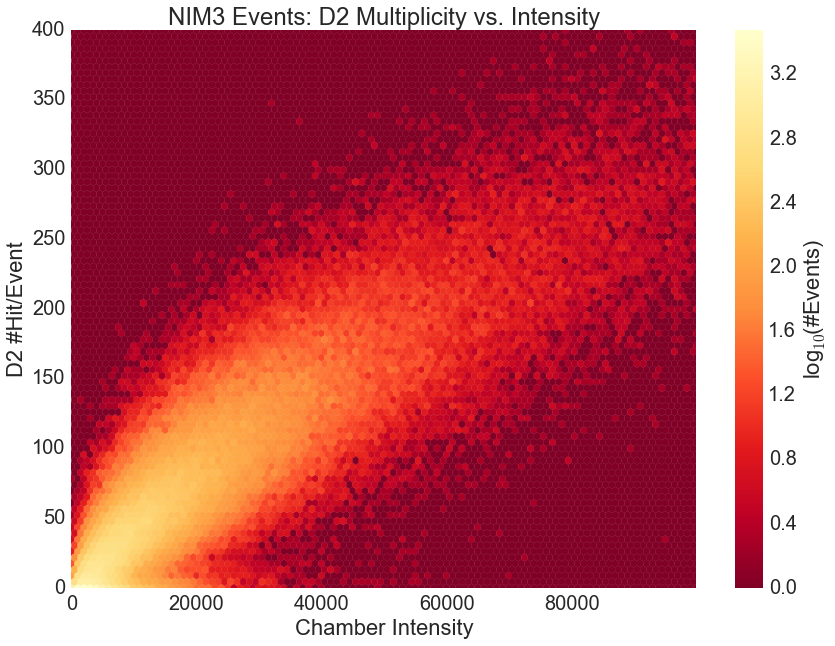
\includegraphics[width=4in]{figures/analysis/NIM3-Int-Mult.png}
	\caption{The linear tendency of detector multiplicity to increase with intensity is observed by looking to unbiased NIM3 events. Here, the occupancy per event of the drift chambers at station 2 are shown as a function of intensity.}
	\label{fig:NIM3-Int-Mult}
\end{figure}

Once the messy and clean samples are prepared, the tracking software is run on them and the two outputs are compared. The first step is to bin the resulting reconstructed dimuons into intensity bins. This binning uses the weights of the dimuons that is assigned by the GMC that created them. The weights are used instead to avoid undue influence on the efficiency from dimuons that are highly unlikely to occur. The value of the bin and its uncertainty are calculated according to Eq.~\ref{eq:gmc-weight}.

For each matching bin, the ratio of $\frac{\#messy}{\#clean}$ values is used to calculate the efficiency of the tracking for that bin. The uncertainty of that efficiency is more complicated, as the relation between the messy and clean samples is of a \emph{binomial} nature. Each dimuon successfully reconstructed in the messy sample represents a \emph{positive} outcome from the number of possible outcomes which is represented by the clean sample. With this kind of relationship, binomial uncertainty calculations must apply. For large enough N number of trials and efficiency $\epsilon\notin \{0,1\}$,
\begin{equation}
\epsilon = \frac{N_+}{N}\ \ ;\ \ \delta\epsilon = \sqrt{\frac{N_+ N_-}{N^3}} = \sqrt{\frac{\epsilon(1-\epsilon)}{N}}
\label{eq:binomial-naive}
\end{equation}
but when weighted trials are involved, things become more complicated in calculating the statistical error. The calculation of this statistical error\cite{blist:binomial} is as follows:
\begin{eqnarray}
	\epsilon & = & \frac{\sum\limits_{i\in+}w_i}{\sum\limits_i w_i} \\
	\delta\epsilon & = & \frac{\sqrt{\sum\limits_{i\in+} w_i^2 \left(\sum\limits_{i\in-} w_i \right)^2 + \
			\sum\limits_{e\in-} w_i^2 \left(\sum\limits_{i\in+} w_i \right)^2}} {\left(\sum\limits_{i}w_i\right)^2}
	\label{eq:binomial-weighted}
\end{eqnarray}
where
\begin{eqnarray}
\sum\limits_{i\in-} w_i & = & \sum\limits_{i\in+}w_i - \sum\limits_{i\in+}w_i \\
\sum\limits_{i\in-} w_i^2 & = & \sum\limits_{i\in+}w_i^2 - \sum\limits_{i\in+}w_i^2 
\end{eqnarray}

For a set of efficiencies, a linear function is fit to the efficiencies. This fit function would then be used to calculate the efficiency for any given dimuon that occurs at any given intensity. The linear parameters are fitted to the data (which is weighted by its statistical uncertainties) by a $\chi^2$-minimization procedure to render a line of best fit along with a confidence interval (Fig.~\ref{fig:keff-all})

\begin{figure}
	\centering
	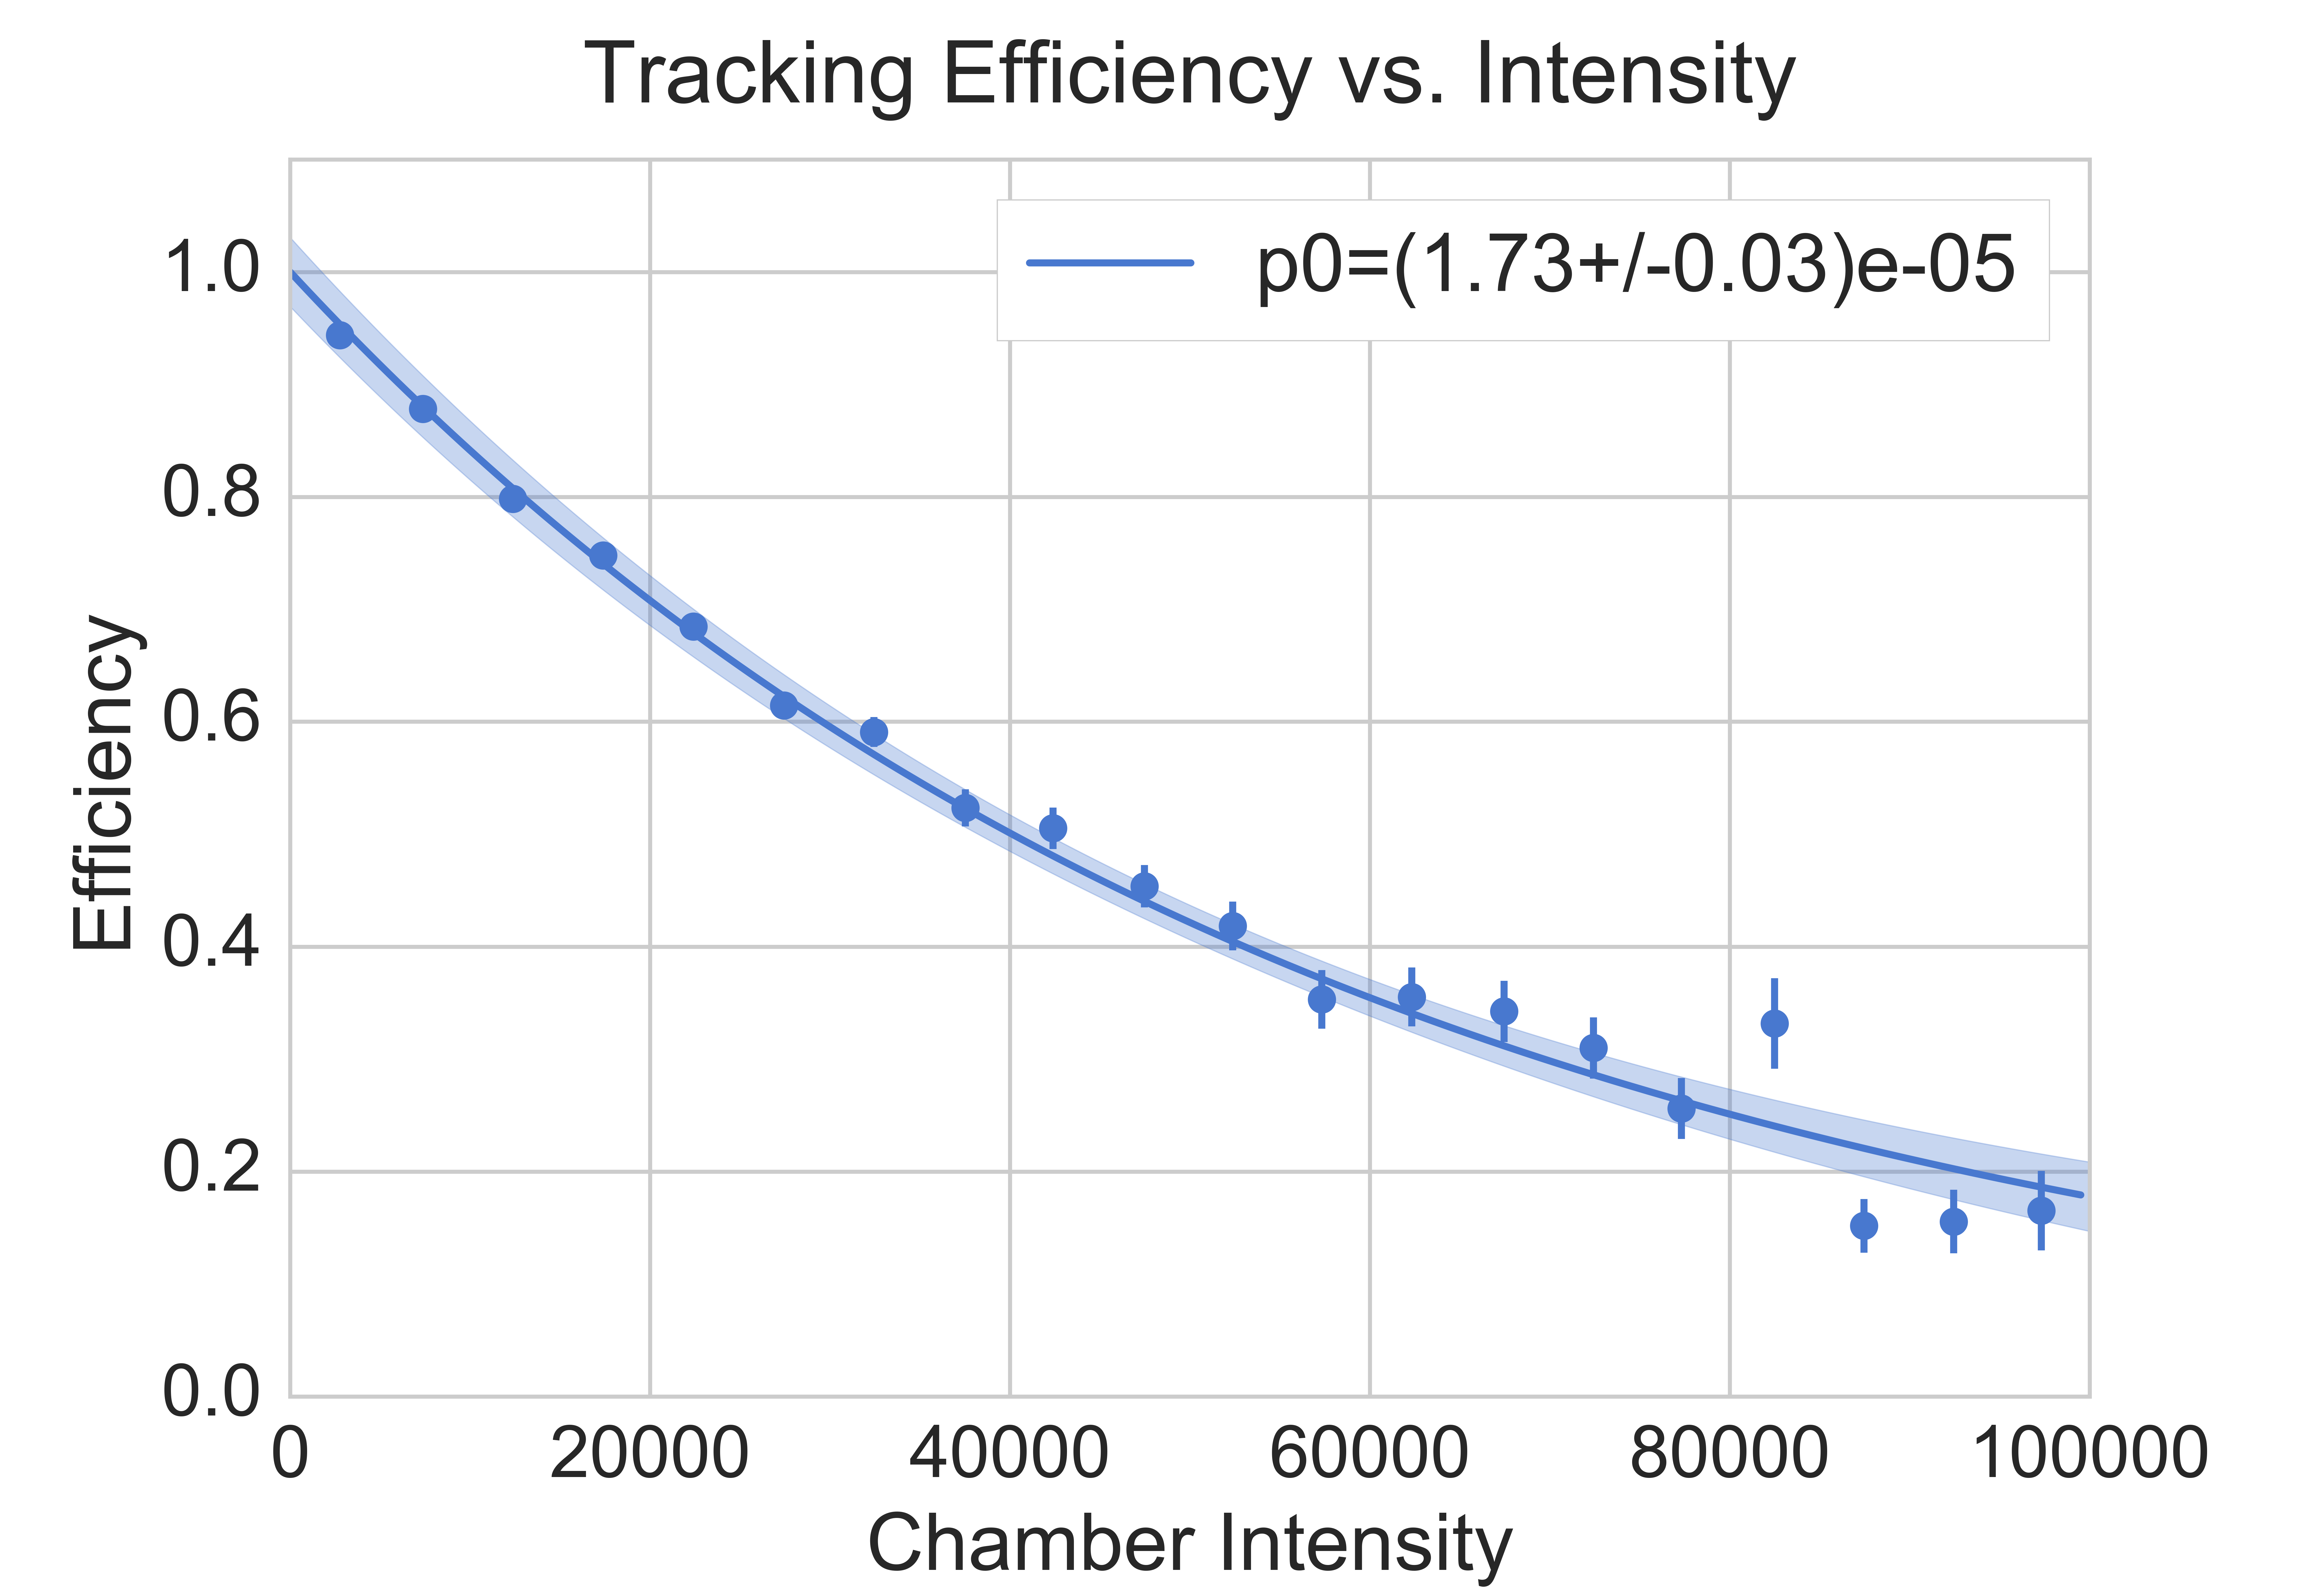
\includegraphics[width=4in]{figures/analysis/all-keff-int.png}
	\caption{The ratio of ``messy'' to ``clean'' dimuon samples from the Deuterium target in Roadset 67 data. This shows the linear relationship of the tracking efficiency to the intensity of the events. The shaded band indicates the 95\% confidence band of the fit.}
	\label{fig:keff-all}
\end{figure}

Further, these fits have a statistically significant kinematic dependence, so it becomes important to unfold the kinematic space and perform this procedure for several kinematic bins in one or more dimensions to assure an accurate efficiency calculation. Of the six defining kinematics of the dimuon, we examine the dependence of the fit on five of them: ($x_1, x_2, p_T, \theta, \phi$), neglecting the azimuthal production angle $\phi_{\gamma^*}$. Each of these five kinematics is divided into three bins (low, medium, high) values to observe on which kinematics the linear fit depends. The results are shown in Figure~\ref{fig:keff-all-kin}.
\begin{figure}
\centering
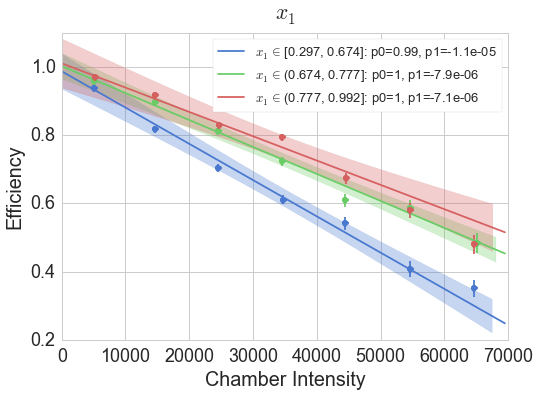
\includegraphics[width=0.49\textwidth]{figures/analysis/x1-keff-int.png}
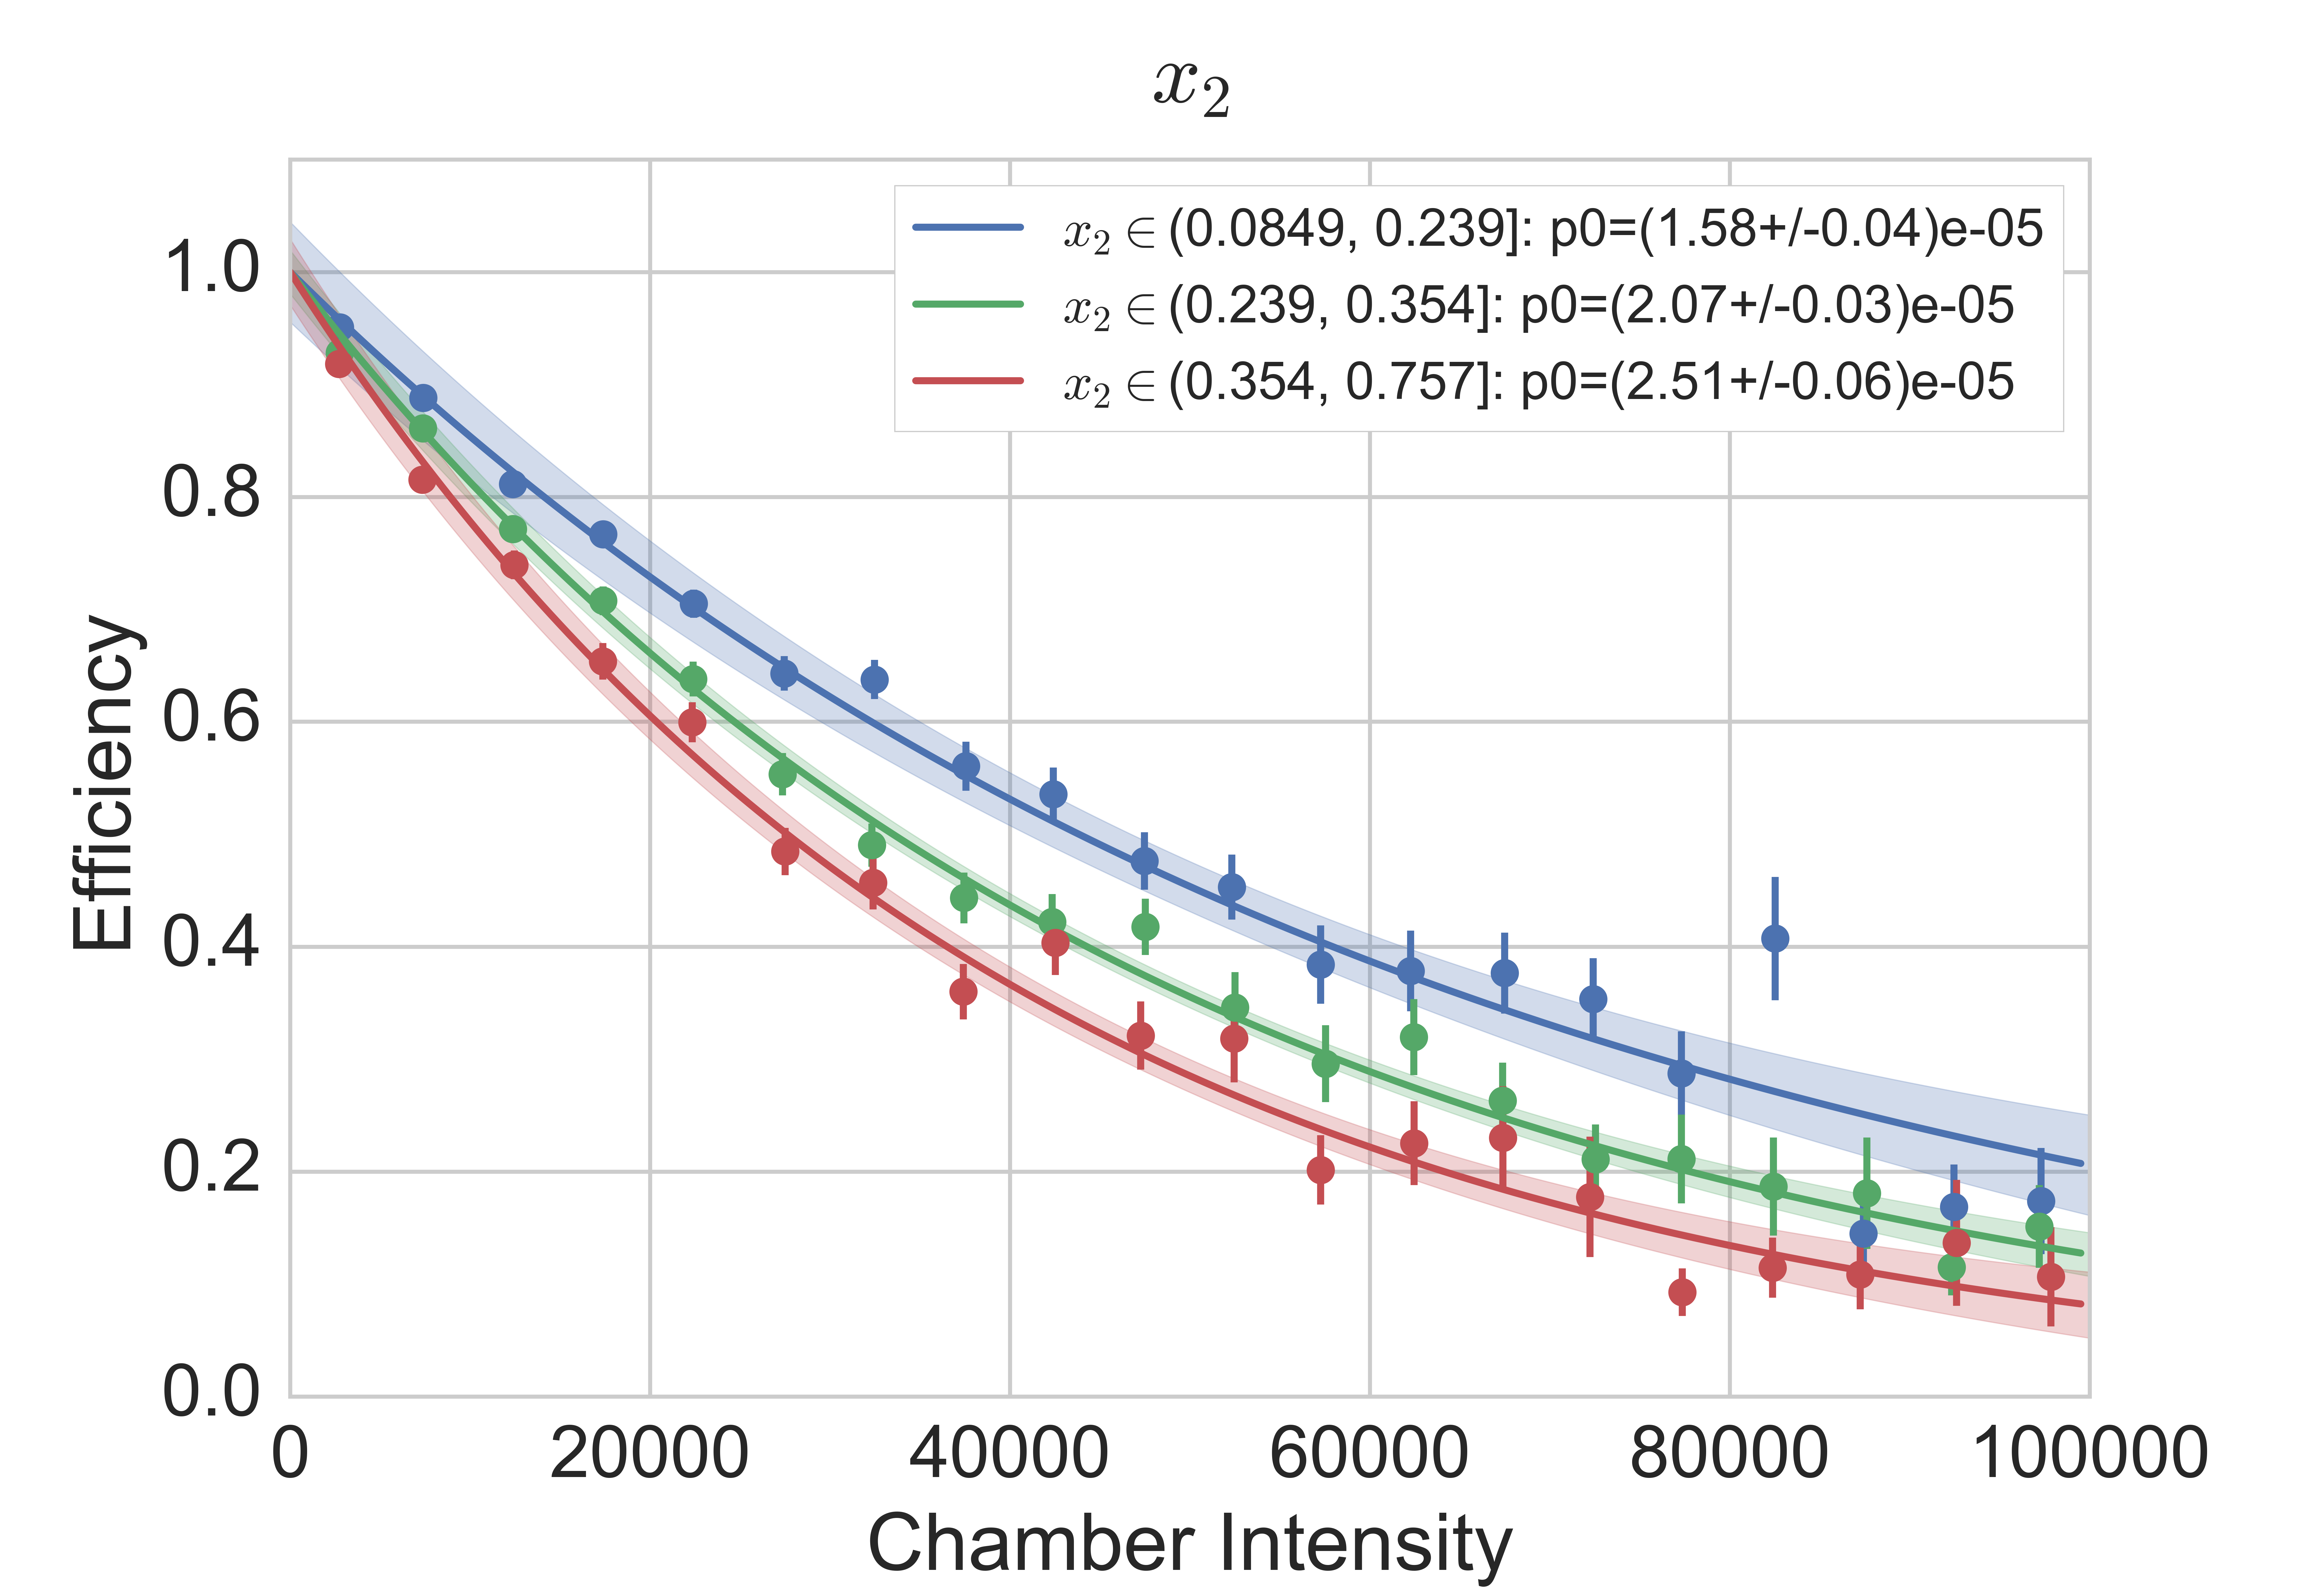
\includegraphics[width=0.49\textwidth]{figures/analysis/x2-keff-int.png} \\
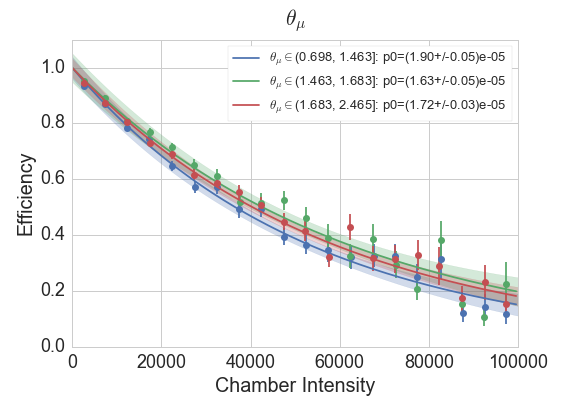
\includegraphics[width=0.49\textwidth]{figures/analysis/theta-keff-int.png}
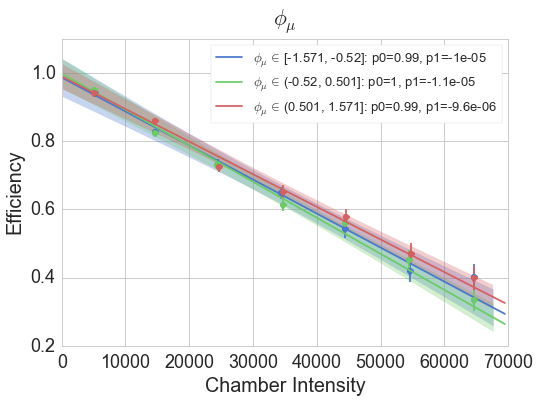
\includegraphics[width=0.49\textwidth]{figures/analysis/phi-keff-int.png} \\
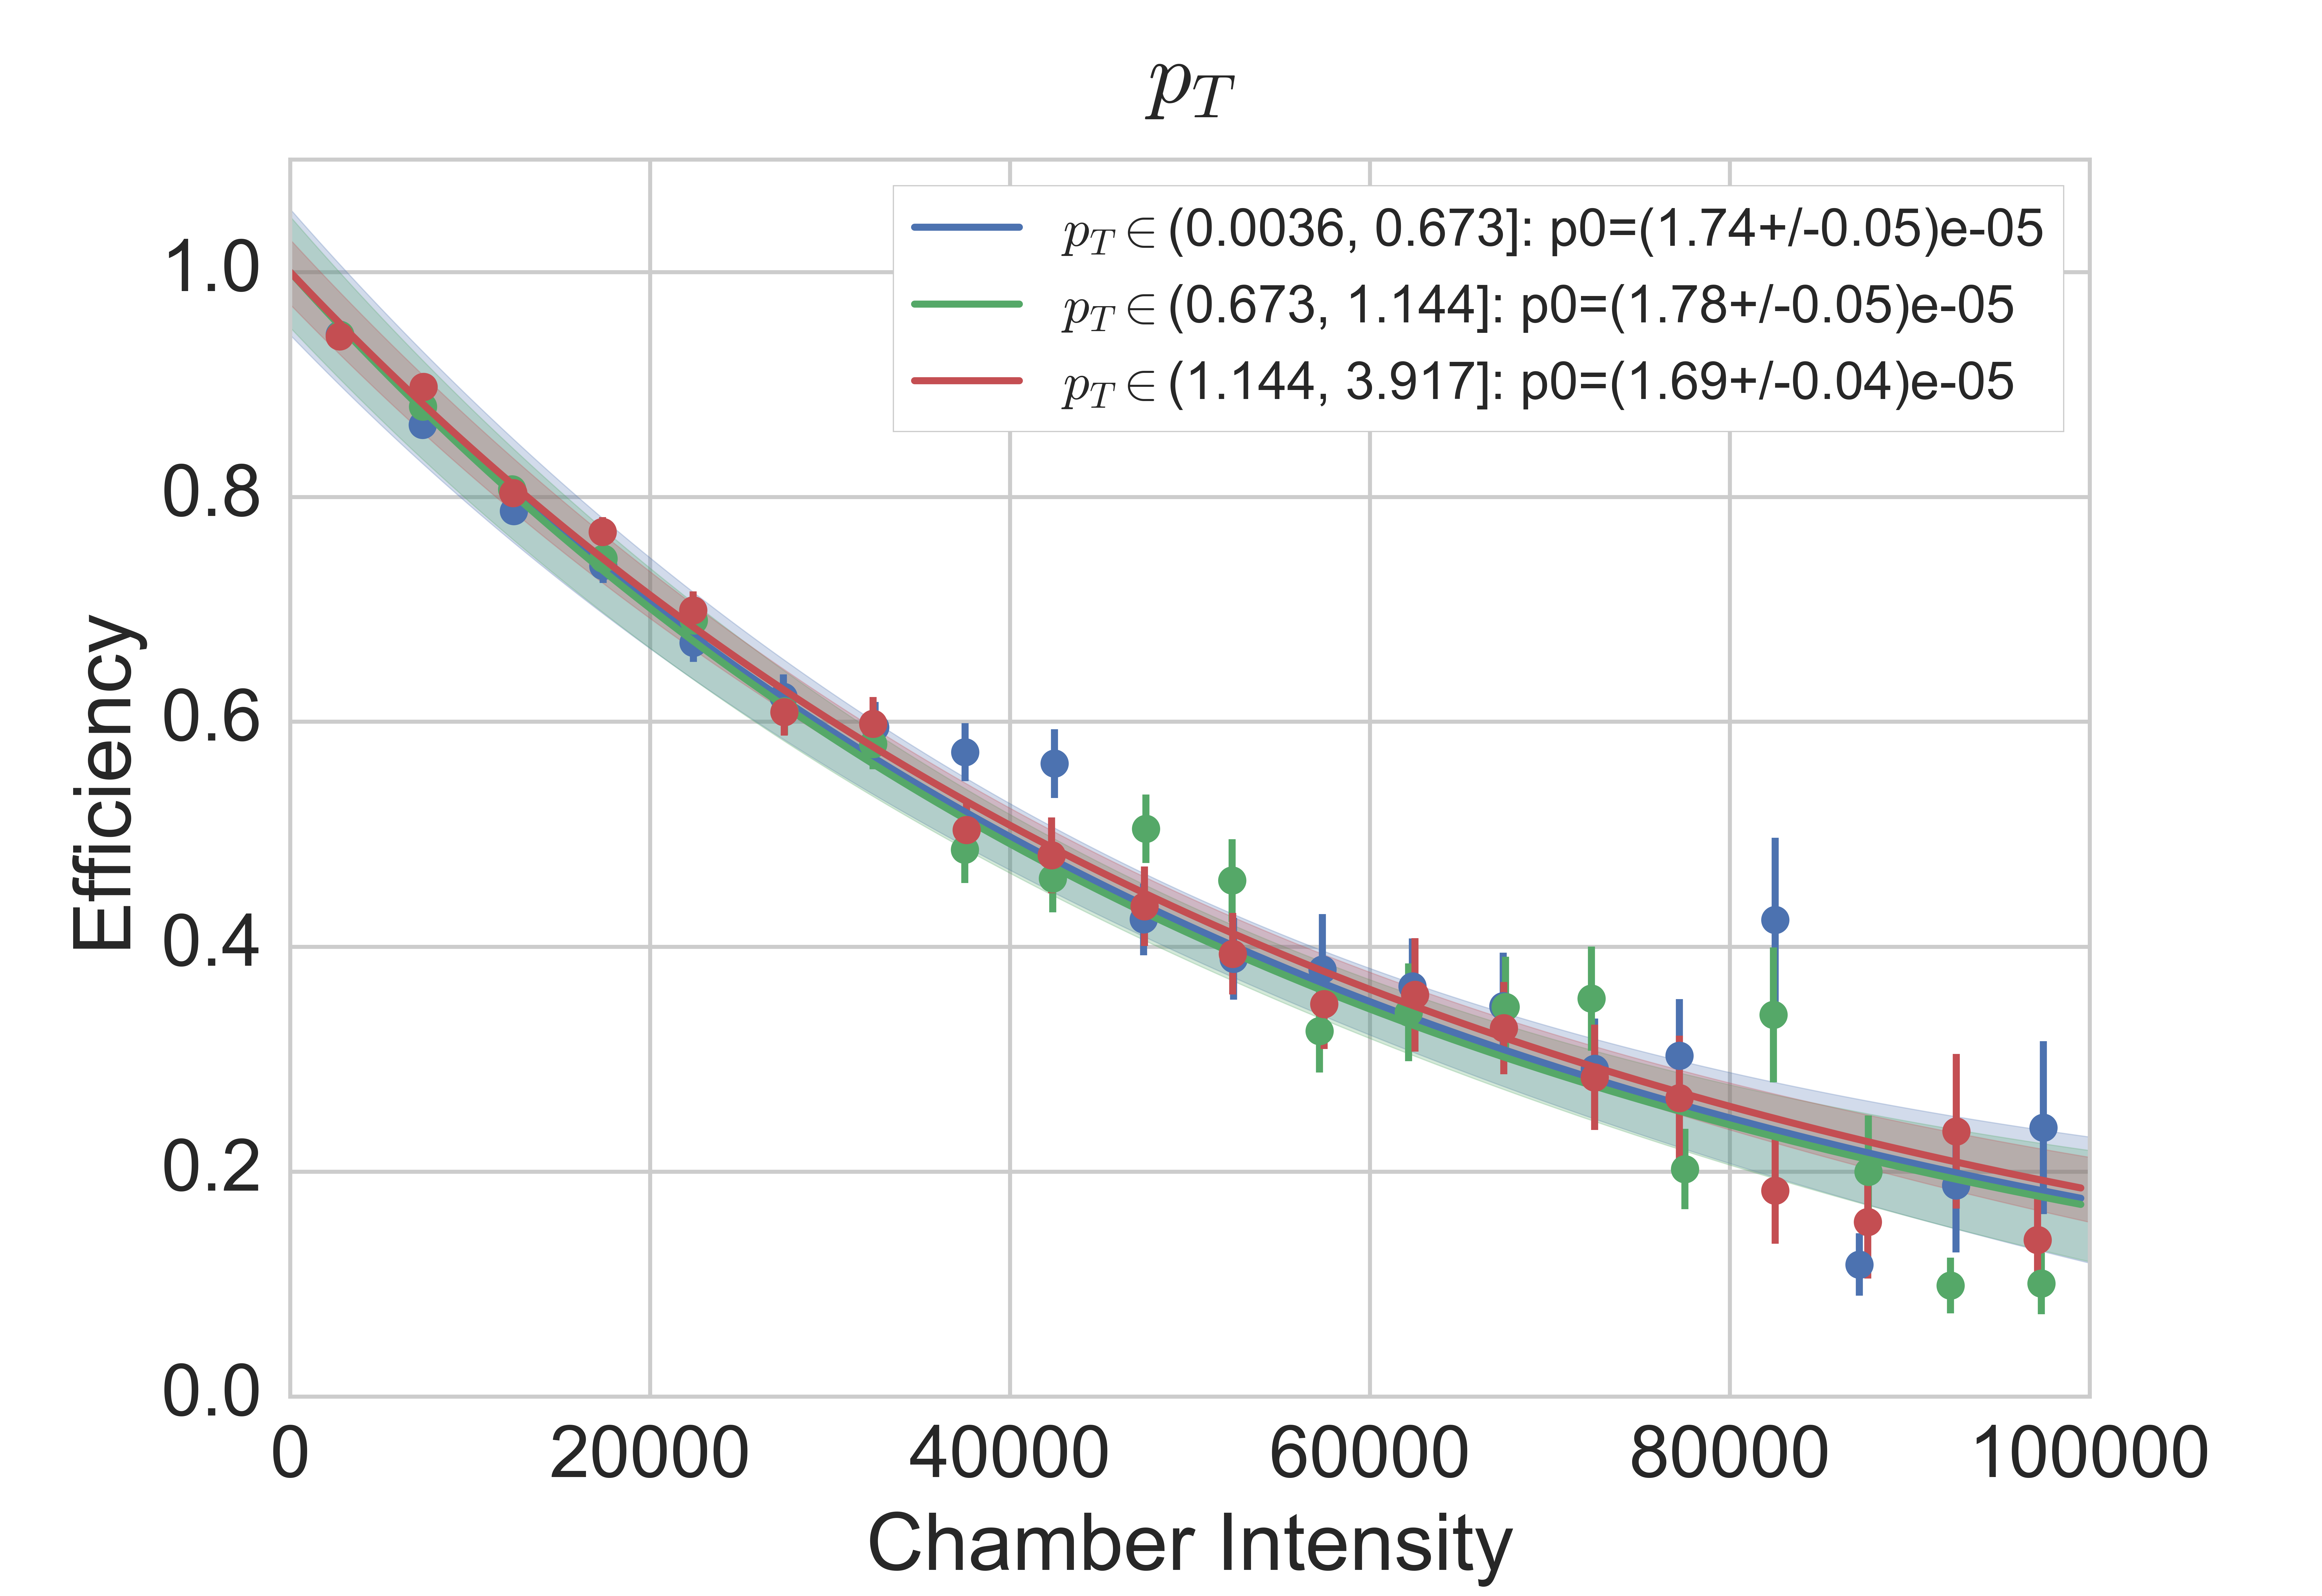
\includegraphics[width=0.49\textwidth]{figures/analysis/pt-keff-int.png}
\caption{Tracking efficiency with the data broken into three statistically equivalent bins in the five primary kinematics, ($x_1, x_2, \theta_\mu, \phi_\mu, p_T$). There appears to be a significant kinematic dependence on $x_1$ and $x_2$.}
\label{fig:keff-all-kin}
\end{figure}
The curves produced seem to indicate that there only exists a kinematic dependence on the $x_1$ and $x_2$ kinematics. If this is the case, then the clean and messy samples can be split two-dimensionally in these two kinematics, and a fit can be made to both variables. When analyzing dimuons, its kinematics can indicate which fit to use to calculate the tracking efficiency based on the intensity of the event, and a weight can be calculated.

But before we come to any clear conclusions, let us investigate two more kinematic phase spaces. We know from the discussion in Chapter 1 that \{$x_1, x_2$\} can be used almost interchangeably with \{$x_F, M_{\gamma^*}$\}, and each of $x_1$ and $x_2$ depend on both $x_F$ and $M_{\gamma^*}$. As such, if only one and not the other shows to influence the tracking efficiency curves, then only that one would be needed for the tracking efficiency correction. We see the behavior of the efficiency curves as a function of $x_F$ and $M_{\gamma^*}$ in Figure~\ref{fig:keff-mass-xf}. It can be concluded that since there is no substantial mass dependence observed, the tracking efficiency has a kinematic dependence solely on $x_F$.

\begin{figure}
	\centering
	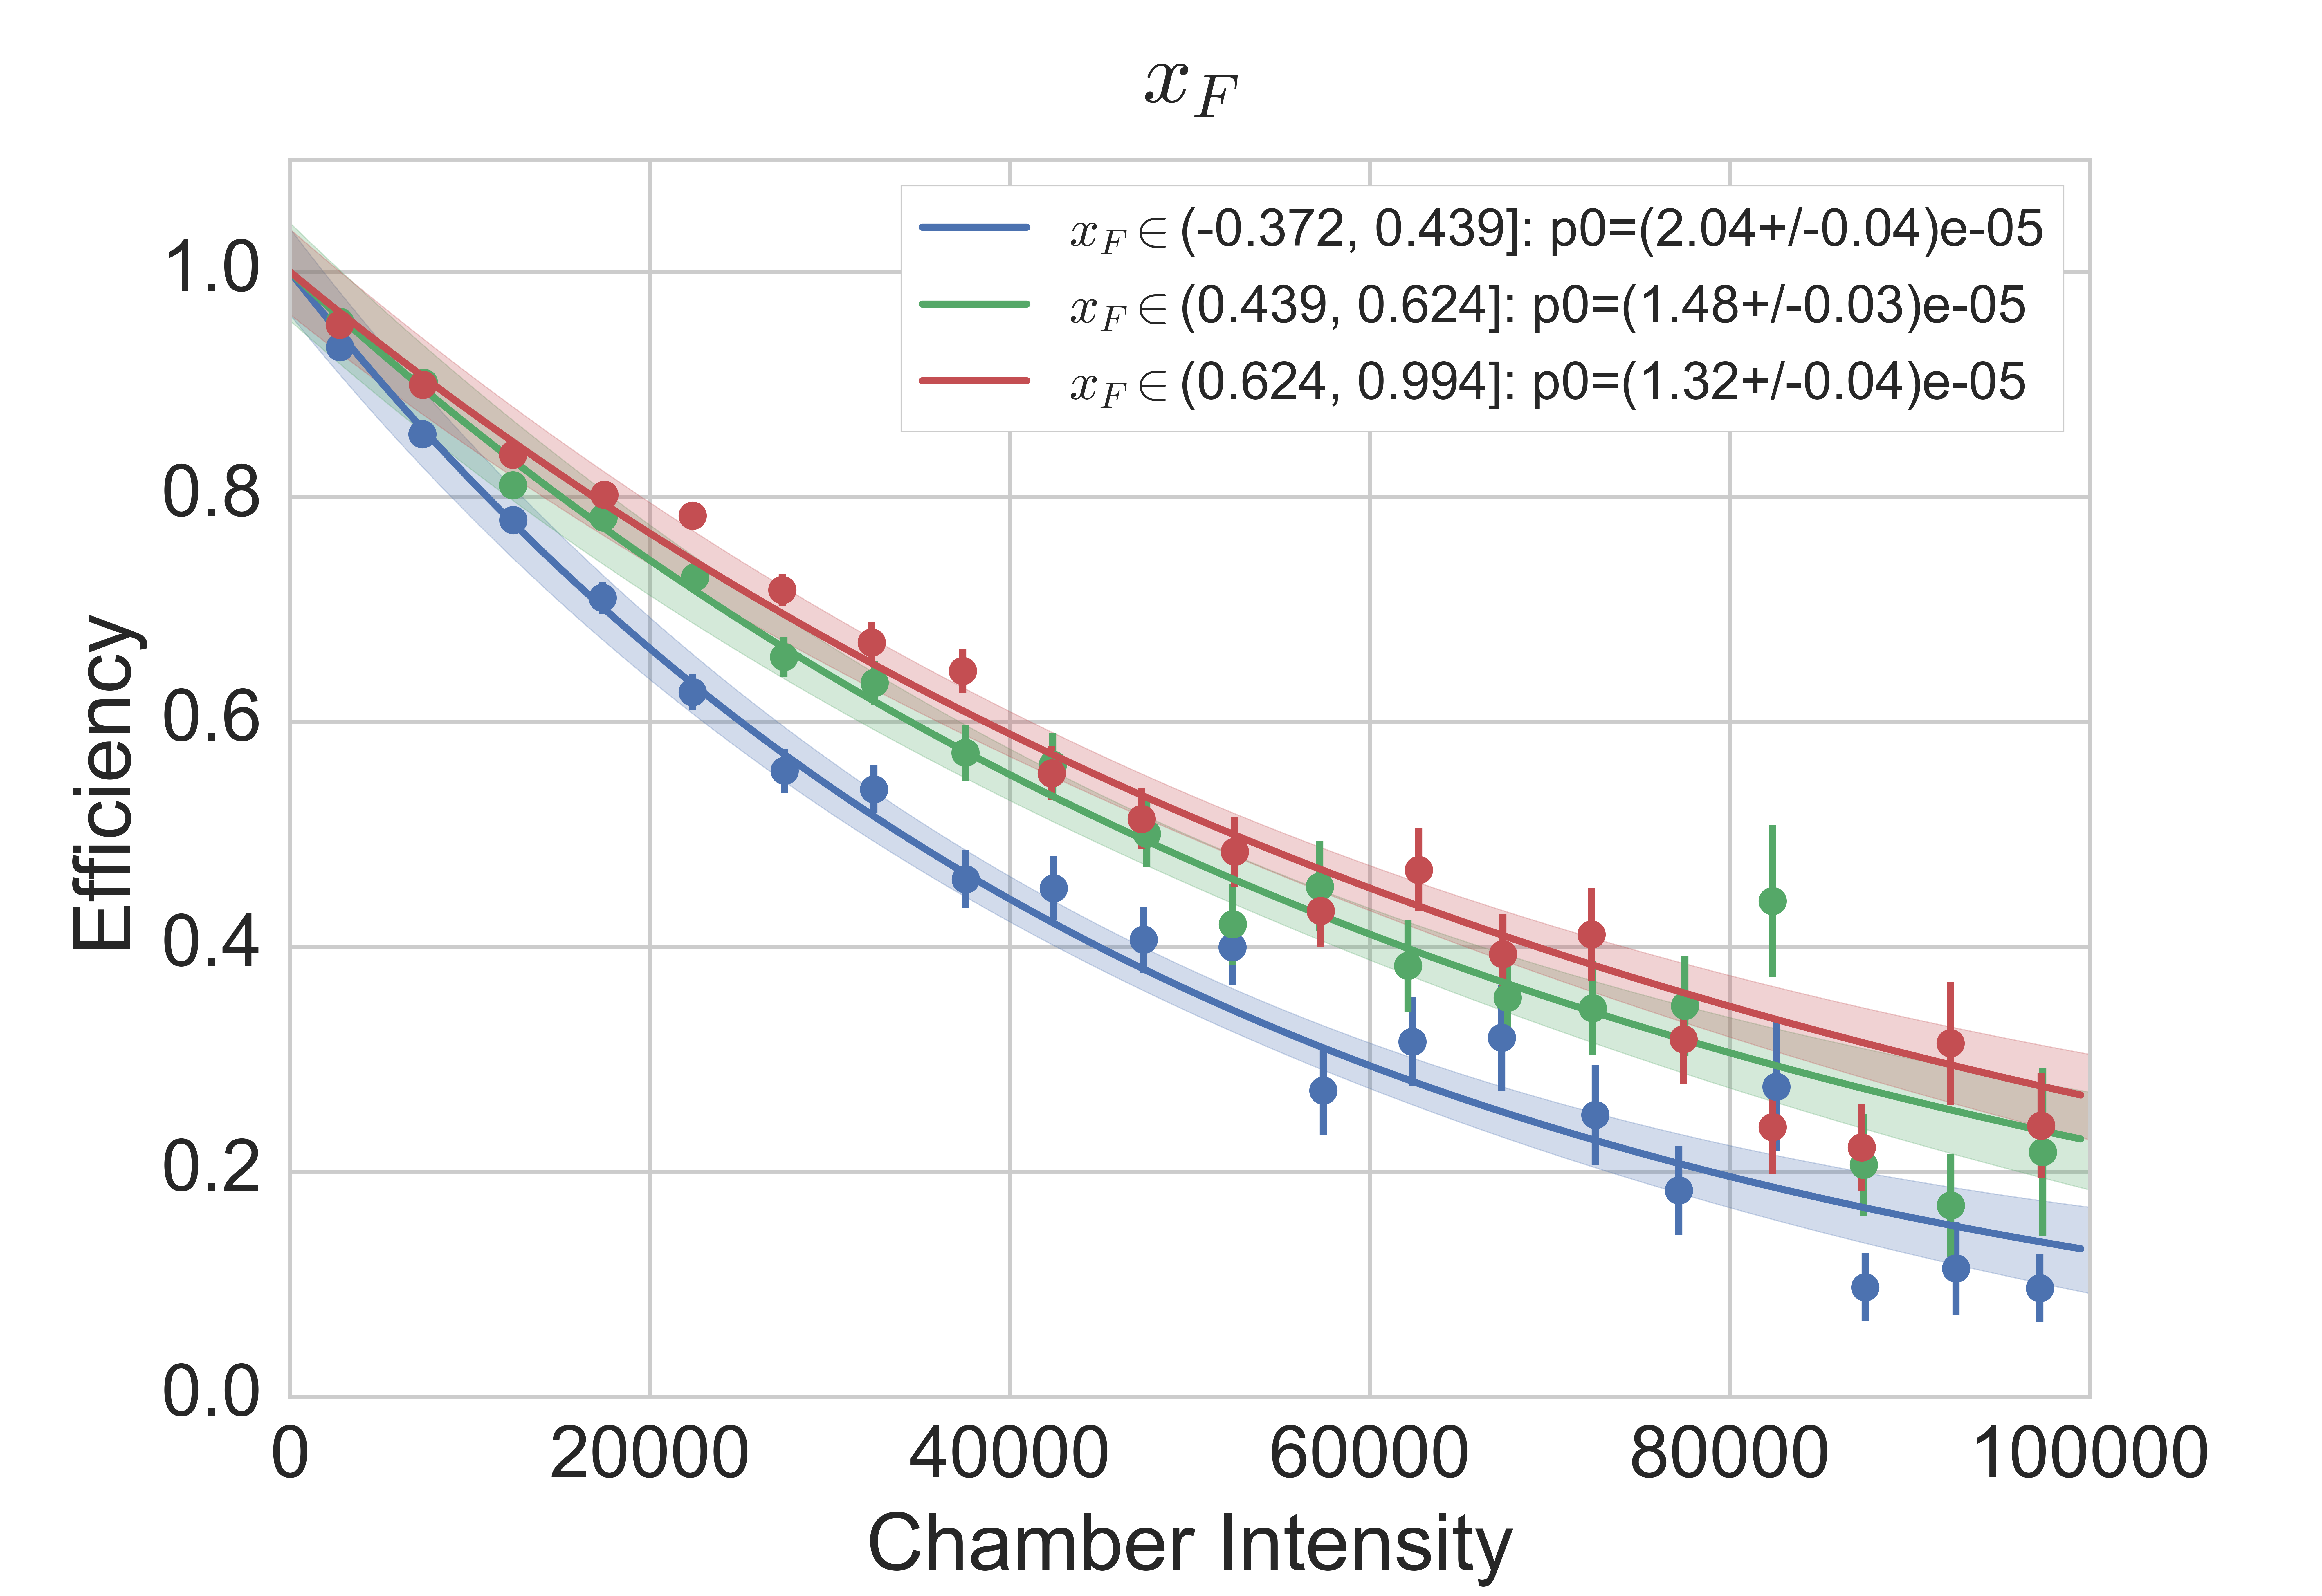
\includegraphics[width=0.49\textwidth]{figures/analysis/xF-keff-int.png}
	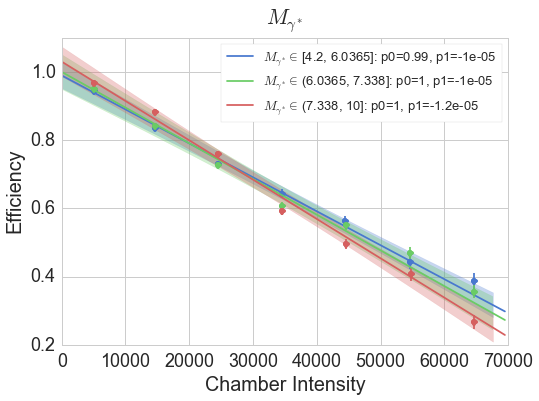
\includegraphics[width=0.49\textwidth]{figures/analysis/mass-keff-int.png}
	\caption{The kinematics $x_F$ and $M_{\gamma^*}$ are investigated. A clear kinematic dependence exists in $x_F$ while $M_{\gamma^*}$ is largely consistent.}
	\label{fig:keff-mass-xf}
\end{figure}

Another consideration is with respect to whether or not there is a target dependence to factor into the correction. For all of the above ``kEfficiency'' plots, only deuterium data is used. The kEfficiency curves for deuterium, hydrogen, carbon, iron, and tungsten can be found on Figure~\ref{fig:keff-target-roadset}. It can be concluded that there is enough of a difference between deuterium, iron, and the rest to justify calculating and applying this correction on a target-by-target basis.
\begin{figure}
	\centering
	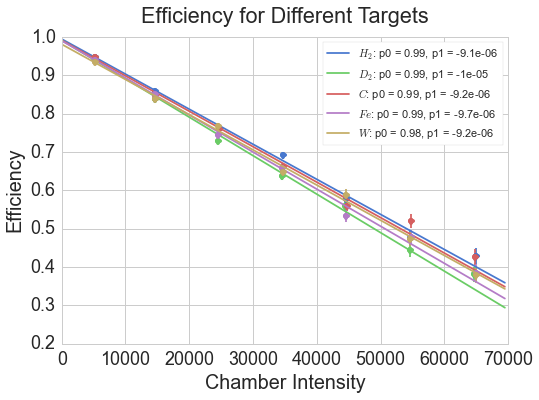
\includegraphics[width=0.49\textwidth]{figures/analysis/target-keff-int.png}
	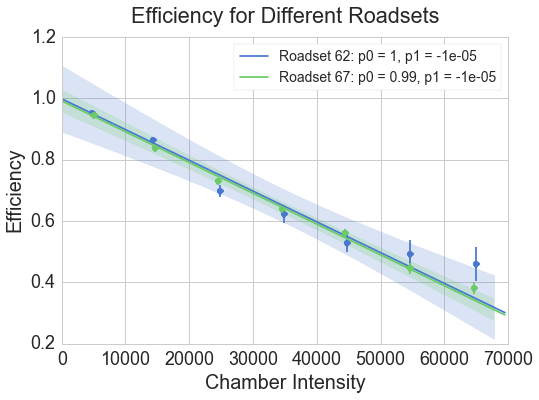
\includegraphics[width=0.49\textwidth]{figures/analysis/roadset-keff-int.png}
	\caption{.}
	\label{fig:keff-target-roadset}
\end{figure}

Also, as a sanity check, there should be no time-dependence of this function. A quick check comparing different sets of data from two different roadsets quickly confirm that there is no such time dependence (Fig.~\ref{fig:keff-target-roadset}).

Depending on the binning of kinematic variables, the result will be intensity-dependent \emph{kEff}$_{t,\bar{x}}(I)$, a set of linear fit functions: one for each target (\emph{t}) and for each kinematic bin ($\bar{x}$), which may be binned in any number of kinematic dimensions.

For each dimuon event \emph{i} of chamber intensity $I_i$, originating from target $t_i$ in kinematic bin $x_i$, create a weight as

\begin{equation}
w_i = \frac{1}{kEff_{t_i, x_i}(I_i)}
\end{equation}

\subsection{The Naive Empty/None Correction}

First a few values must be defined. An overall efficiency based on 'contributions' from the Empty/None background can be defined as

\begin{equation}
\epsilon_b = 1 - \frac{Y_b/p_b}{Y_t/p_t} = 1 - \left(\frac{p_t}{p_b}\right) \left( \frac{Y_b}{Y_t} \right)
\end{equation}

where Y is the dimuon \emph{yield} from a given target and \emph{p} is the integrated ``live proton'' count for the same given target. Here, $b \in \{Empty,\ None\}$ and $t\in\{H,\ D,\ C,\ Fe,\ W\}$. It is yet to be conclusively decided by the collaboration whether or not the Empty and None targets are to be combined for these calculations.

The next step is to adjust the yields with the \emph{kEff}$_{t,\bar{x}}(I)$:

\begin{equation}
Y_a \rightarrow Y_a^\prime = \sum_{i:i_t=a} \frac{1}{kEff_{t_i, x_i}(I_i)}
\end{equation}

The yield efficiency when factoring in background then becomes

\begin{equation}
\epsilon^\prime_b = 1 - \left(\frac{p_t}{p_b}\right) \left( \frac{Y^\prime_b}{Y^\prime_t} \right)
\end{equation}

\subsection{The Empty/None vs. Intensity Curve}


\subsection{A New Background Correction}

With the Empty/None vs. Intensity Curve \emph{C(I)}, we can apply a more sophisticated correction. With C(I), we can make an expression for the background contribution to the yields of a given target:

\begin{equation}
p_t \left( \frac{Y^\prime_b}{p_b} \right) = \sum_{i:i_t=t} \frac{D\cdot C(I_i)}{kEff_{t_i, x_i}(I_i)}
\end{equation}
where D is a normalization constant defined in such a way that $D \cdot C(I)$ is the \% chance that a given dimuon from a target actually came from the Empty/None background. D can be calculated as
\begin{eqnarray}
D & = & \frac{1}{F} Y^\prime_b \left( \frac{p_t}{p_b} \right) \\
F & = &\sum_{i: i_t=t} \frac{C(I_i)}{kEff_{t_i, x_i}(I_i)}
\end{eqnarray}

The new intensity-dependent efficiency can now be defined as

\begin{equation}
(\epsilon_b^\prime)_i = 1 - D \cdot C(I_i)
\end{equation}

\section{Rate Dependence and Combinatorial Background Correction}



\section{Empty/None Target Background Subtraction}



\section{Dimuon Yield Ratios}



\section{$ld_2$ Contamination Correction}



\section{Isoscalar Corrections for $^{183}W$ and $^{56}Fe$}


